%%%%%%%%%%%%%%%%%%%%%%%%%%%%%%%%%%%%%%%%%%%%%%%%%%%%%%%%%%%%%%%%%%%%%%%%%%%%%%%%%%%%%%%%%%%%%%%%%%%%%%%%%%%%%%%%%%%%%%%%%%%%%%%%%%%%%%%%%%%%%%%%%%%%%%%%%%%%%%%%%%%%%%%%%%%%%%%%%%%%%%%%%%%%
% Written By Michael Brodskiy
% Class: AP Chemistry
% Professor: J. Morgan
%%%%%%%%%%%%%%%%%%%%%%%%%%%%%%%%%%%%%%%%%%%%%%%%%%%%%%%%%%%%%%%%%%%%%%%%%%%%%%%%%%%%%%%%%%%%%%%%%%%%%%%%%%%%%%%%%%%%%%%%%%%%%%%%%%%%%%%%%%%%%%%%%%%%%%%%%%%%%%%%%%%%%%%%%%%%%%%%%%%%%%%%%%%%

\documentclass[12pt]{article} 
\usepackage{alphalph}
\usepackage[utf8]{inputenc}
\usepackage[russian,english]{babel}
\usepackage{titling}
\usepackage{amsmath}
\usepackage{graphicx}
\usepackage{enumitem}
\usepackage{amssymb}
\usepackage[super]{nth}
\usepackage{expl3}
\usepackage[version=4]{mhchem}
\usepackage{hpstatement}
\usepackage{rsphrase}
\usepackage{everysel}
\usepackage{ragged2e}
\usepackage{geometry}
\usepackage{fancyhdr}
\usepackage{cancel}
\usepackage{siunitx}
\usepackage{chemfig}
\geometry{top=1.0in,bottom=1.0in,left=1.0in,right=1.0in}
\newcommand{\subtitle}[1]{%
  \posttitle{%
    \par\end{center}
    \begin{center}\large#1\end{center}
    \vskip0.5em}%

}
\newcommand{\orbital}[2]{{%
    \def\+{\big|\hspace{-2pt}\overline{\underline{\hspace{2pt}\upharpoonleft}}}%
    \def\-{\overline{\underline{\downharpoonright\hspace{2pt}}}\hspace{-2pt}\big|}%
    \def\0{\big|\hspace{-2pt}\overline{\underline{\phantom{\hspace{2pt}\downharpoonright}}}}%
    \def\1{\overline{\underline{\phantom{\downharpoonright\hspace{2pt}}}}\hspace{-2pt}\big|}%
  \setlength\tabcolsep{0pt}% remove extra horizontal space from tabular
  \begin{tabular}{c}$#2$\\[2pt]#1\end{tabular}%
}}
\DeclareSIUnit\Molar{\textsc{m}}
\DeclareSIUnit\atm{\textsc{atm}}
\DeclareSIUnit\torr{\textsc{torr}}
\DeclareSIUnit\psi{\textsc{psi}}
\DeclareSIUnit\bar{\textsc{bar}}
\DeclareSIUnit\Celsius{\textsc{C}}
\usepackage{hyperref}
\hypersetup{
colorlinks=true,
linkcolor=blue,
filecolor=magenta,      
urlcolor=blue,
citecolor=blue,
}

\urlstyle{same}


\title{Chapter 8 $-$ Thermochemistry}
\date{\today}
\author{Michael Brodskiy\\ \small Instructor: Mr. Morgan}

% Mathematical Operations:

% Sum: $$\sum_{n=a}^{b} f(x) $$
% Integral: $$\int_{lower}^{upper} f(x) dx$$
% Limit: $$\lim_{x\to\infty} f(x)$$

\begin{document}

\maketitle

\begin{itemize}

  \item Reactions either absorb heat or release it:

    \begin{enumerate}

      \item Exothermic Reaction $-$ Releases heat

      \item Endothermic Reaction $-$ Intakes heat

    \end{enumerate}

  \item $q=cm\Delta T$, where $c$ is the specific heat and $q$ is the heat/energy
    
  \item Units of specific heat are $\left[ \frac{\si{\joule}}{\si{\gram\Celsius}} \right]$

  \item Enthalpy ($\Delta H$) $-$ Reaction heat content. If $\Delta H<0$ the reaction is exothermic, but if $\Delta H>0$, the reaction is endothermic.

  \item $\Delta H$ for a reaction is equal but opposite in sign for reverse.

  \item Hess's Law $-$ $\Delta H$ for a reaction is same whether it occurs directly or in a series.

    \begin{enumerate}

      \item The enthalpy is the same for the following reactions:

        $$\ce{A}\rightarrow\ce{D}$$

        $$\ce{A}\rightarrow\ce{B}\rightarrow\ce{C}\rightarrow\ce{D}$$

    \end{enumerate}

  \item The Enthalpy of formations, $\Delta H_f$, is the energy to form compounds: $\Delta H=\sum$ products $-\sum$ reactants

    \begin{enumerate}

      \item Single, non-charged atoms (ex. \ce{O2}) equal zero

    \end{enumerate}

  \item $\Delta H$ may also be calculated through bond energies. $\Delta H=$ Break $-$ Make.

  \item First line, heat of fusion, second line, heat of vaporization (it takes more energy to boil something than to melt something)

    \begin{figure}[H]
      \centering
      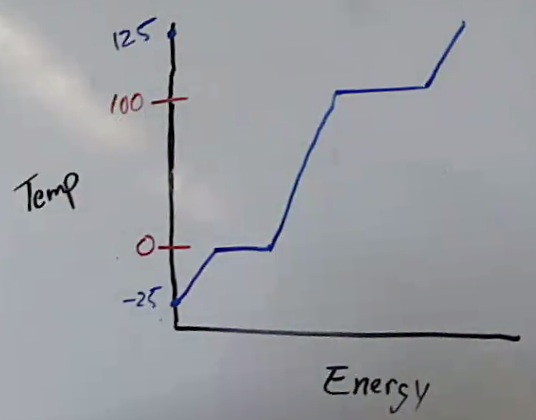
\includegraphics{Figures/HeatCooling.png}
      \caption{Heating/Cooling Curve for \ce{H2O}}
      \label{fig:1}
    \end{figure}

  \item Energy is only given off when a bond is made. It takes energy to break bonds.

\end{itemize}

\end{document}

